% The gate count of one oracle call, counted off the unfolded strip of
% fig1-unfold.tex: the same boxes, each with its gate cost beneath, so the
% formula under the figure reads as a count of boxes.  Rendered to an SVG
% of paths by the Makefile.
\documentclass[dvisvgm]{standalone}
\usepackage{amsmath,amssymb}
\usepackage{tikz}
\definecolor{deckgreen}{HTML}{4D8C55}
\tikzset{phase/.style={draw=deckgreen, fill=deckgreen!12, rounded corners=2pt,
  line width=0.4mm, minimum width=1.25cm, minimum height=0.6cm, font=\footnotesize}}
\begin{document}
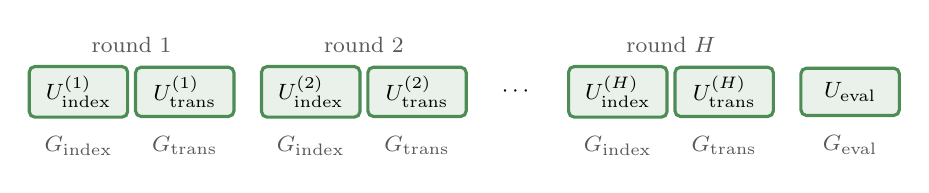
\begin{tikzpicture}[
  lbl/.style={font=\footnotesize},
  cost/.style={font=\footnotesize, text=gray!70!black},
]
  \node[phase] (i1) at (-1.6, 0)  {$U^{(1)}_{\mathrm{index}}$};
  \node[phase] (t1) at (-0.25, 0) {$U^{(1)}_{\mathrm{trans}}$};
  \node[phase] (i2) at (1.35, 0)  {$U^{(2)}_{\mathrm{index}}$};
  \node[phase] (t2) at (2.7, 0)   {$U^{(2)}_{\mathrm{trans}}$};
  \node[lbl]        at (3.975, 0) {$\cdots$};
  \node[phase] (iH) at (5.25, 0)  {$U^{(H)}_{\mathrm{index}}$};
  \node[phase] (tH) at (6.6, 0)   {$U^{(H)}_{\mathrm{trans}}$};
  \node[phase] (ev) at (8.2, 0)   {$U_{\mathrm{eval}}$};

  \node[cost] at (-0.925, 0.6) {round 1};
  \node[cost] at (2.025, 0.6)  {round 2};
  \node[cost] at (5.925, 0.6)  {round $H$};

  \foreach \n in {i1, i2, iH} { \node[cost, below=3pt] at (\n.south) {$G_{\mathrm{index}}$}; }
  \foreach \n in {t1, t2, tH} { \node[cost, below=3pt] at (\n.south) {$G_{\mathrm{trans}}$}; }
  \node[cost, below=3pt] at (ev.south) {$G_{\mathrm{eval}}$};
\end{tikzpicture}
\end{document}
